% chapters/chapter2/2_6_trajectory.tex
% !TeX root=../../main.tex

\section{برنامه‌ریز مسیر سینماتیکی}
\label{sec:trajectory_planner}

یکی از چالش‌های بنیادین در کنترل سیستم‌های زیرفعال با محدودیت‌های سخت فیزیکی، نحوه اعمال موقعیت هدف به سیستم است. در معماری‌های پایه، معمولاً موقعیت نهایی به صورت یک ورودی پله (\lr{Step Input}) به سیستم اعمال می‌شود. اعمال یک‌باره خطای بزرگ موقعیت ($e = x_{ref} - x_0$) در لحظه شروع حرکت، کنترل‌کننده را وادار می‌کند تا برای کاهش سریع خطا، حداکثر نیروی ممکن را درخواست کند. این امر به صورت اجتناب‌ناپذیری به اشباع عملگرها (\lr{Actuator Saturation})، اعمال شوک‌های مکانیکی به سازه و نقض فرض‌های خطی‌سازی در زوایای کوچک می‌انجامد. در جابجایی‌های بزرگ، این رفتار خشن باعث خروج سریع آونگ از محدوده پایدار و بروز ناپایداری‌های فاز می‌شود.

برای غلبه بر این چالش ساختاری، موقعیت هدف نه به صورت یک جهش ناگهانی، بلکه در قالب یک مسیر پیوسته و سینماتیکی تولید می‌گردد. به همین منظور، از یک برنامه‌ریز مسیر (\lr{Trajectory Planner}) بر مبنای منحنی نرم (\lr{S-Curve}) استفاده شده است. این واحد با دریافت موقعیت اولیه و نهایی، یک پروفایل حرکتی مطلوب تولید می‌کند که در هر لحظه، مرجع موقعیت ($x_{ref}$)، سرعت ($\dot{x}_{ref}$) و شتاب ($\ddot{x}_{ref}$) را برای کالسکه تعیین می‌کند.

منطق ریاضی برنامه‌ریز مسیر بر پایه رعایت دقیق قیود سینماتیکی سیستم بنا شده است. در این راستا، حداکثر سرعت مجاز کالسکه $v_{\max} = 1.0$ متر بر ثانیه و حداکثر شتاب آن $a_{\max} = 2.0$ متر بر مجذور ثانیه در نظر گرفته شده است. انتخاب این مقادیر بر مبنای دو عامل کلیدی صورت گرفته است: نخست، حفظ نیروی درخواستی در محدوده ظرفیت نامی موتورهای محرک و جلوگیری از پدیده اشباع؛ و دوم، محدود ساختن شتاب انتقالی کالسکه برای جلوگیری از تحریک بیش از حد دینامیک زیرفعال (آونگ) و حفظ زاویه نوسان در کران‌های ایمن.

\subsection{توسعه روابط ریاضی مسیر مرجع}
برای تضمین پیوستگی در سرعت و شتاب (جلوگیری از ضربه یا \lr{Jerk} ناگهانی)، از یک چندجمله‌ای مرتبه ۵ برای تولید پروفایل حرکتی استفاده می‌شود. زمان کل سفر ($T$) بر اساس قیود سرعت و شتاب و همچنین دوره تناوب طبیعی آونگ ($T_p = 2\pi\sqrt{l_0/g}$) محاسبه می‌شود تا مانور حرکتی به اندازه کافی نرم باشد:
\begin{equation}
    T = \max \left( \frac{15}{8} \frac{D}{v_{\max}}, \sqrt{\frac{5.77 D}{a_{\max}}}, 1.5 T_p \right)
\end{equation}
که در آن $D$ مقدار مطلق جابجایی است. با تعریف متغیر زمان نرمالایز شده $\tau = t/T$، معادله موقعیت و مشتقات آن به صورت زیر استخراج می‌شوند:
\begin{equation}
    s(\tau) = 10\tau^3 - 15\tau^4 + 6\tau^5
\end{equation}
\begin{equation}
    \dot{s}(\tau) = \frac{1}{T} \left( 30\tau^2 - 60\tau^3 + 30\tau^4 \right)
\end{equation}
\begin{equation}
    \ddot{s}(\tau) = \frac{1}{T^2} \left( 60\tau - 180\tau^2 + 120\tau^3 \right)
\end{equation}
این ساختار ریاضی تضمین می‌کند که سرعت و شتاب در لحظه شروع ($t = 0$) و پایان ($t = T$) مسیر دقیقاً برابر صفر باشند.

علاوه بر تولید مسیر مرجع هندسی، این برنامه‌ریز یک سیگنال فیدفوروارد تحلیلی ($F_{ff}$) نیز تولید می‌کند. وظیفه این سیگنال، تأمین نیروی خالص مورد نیاز برای غلبه بر اینرسی و اصطکاک کالسکه است تا بار اصلی از دوش کنترل‌کننده فیدبک برداشته شود:
\begin{equation}
    F_{ff} = (M + m) a_{ref} + b_c v_{ref}
\end{equation}

کدهای پیاده‌سازی این برنامه‌ریز و محاسبات سینماتیکی آن در محیط نرم‌افزار متلب، به طور کامل در برنامه \ref{code:traj_generator} در پیوست \ref{app:matlab_codes} ارائه شده است.

\begin{figure}[htbp]
    \centering
    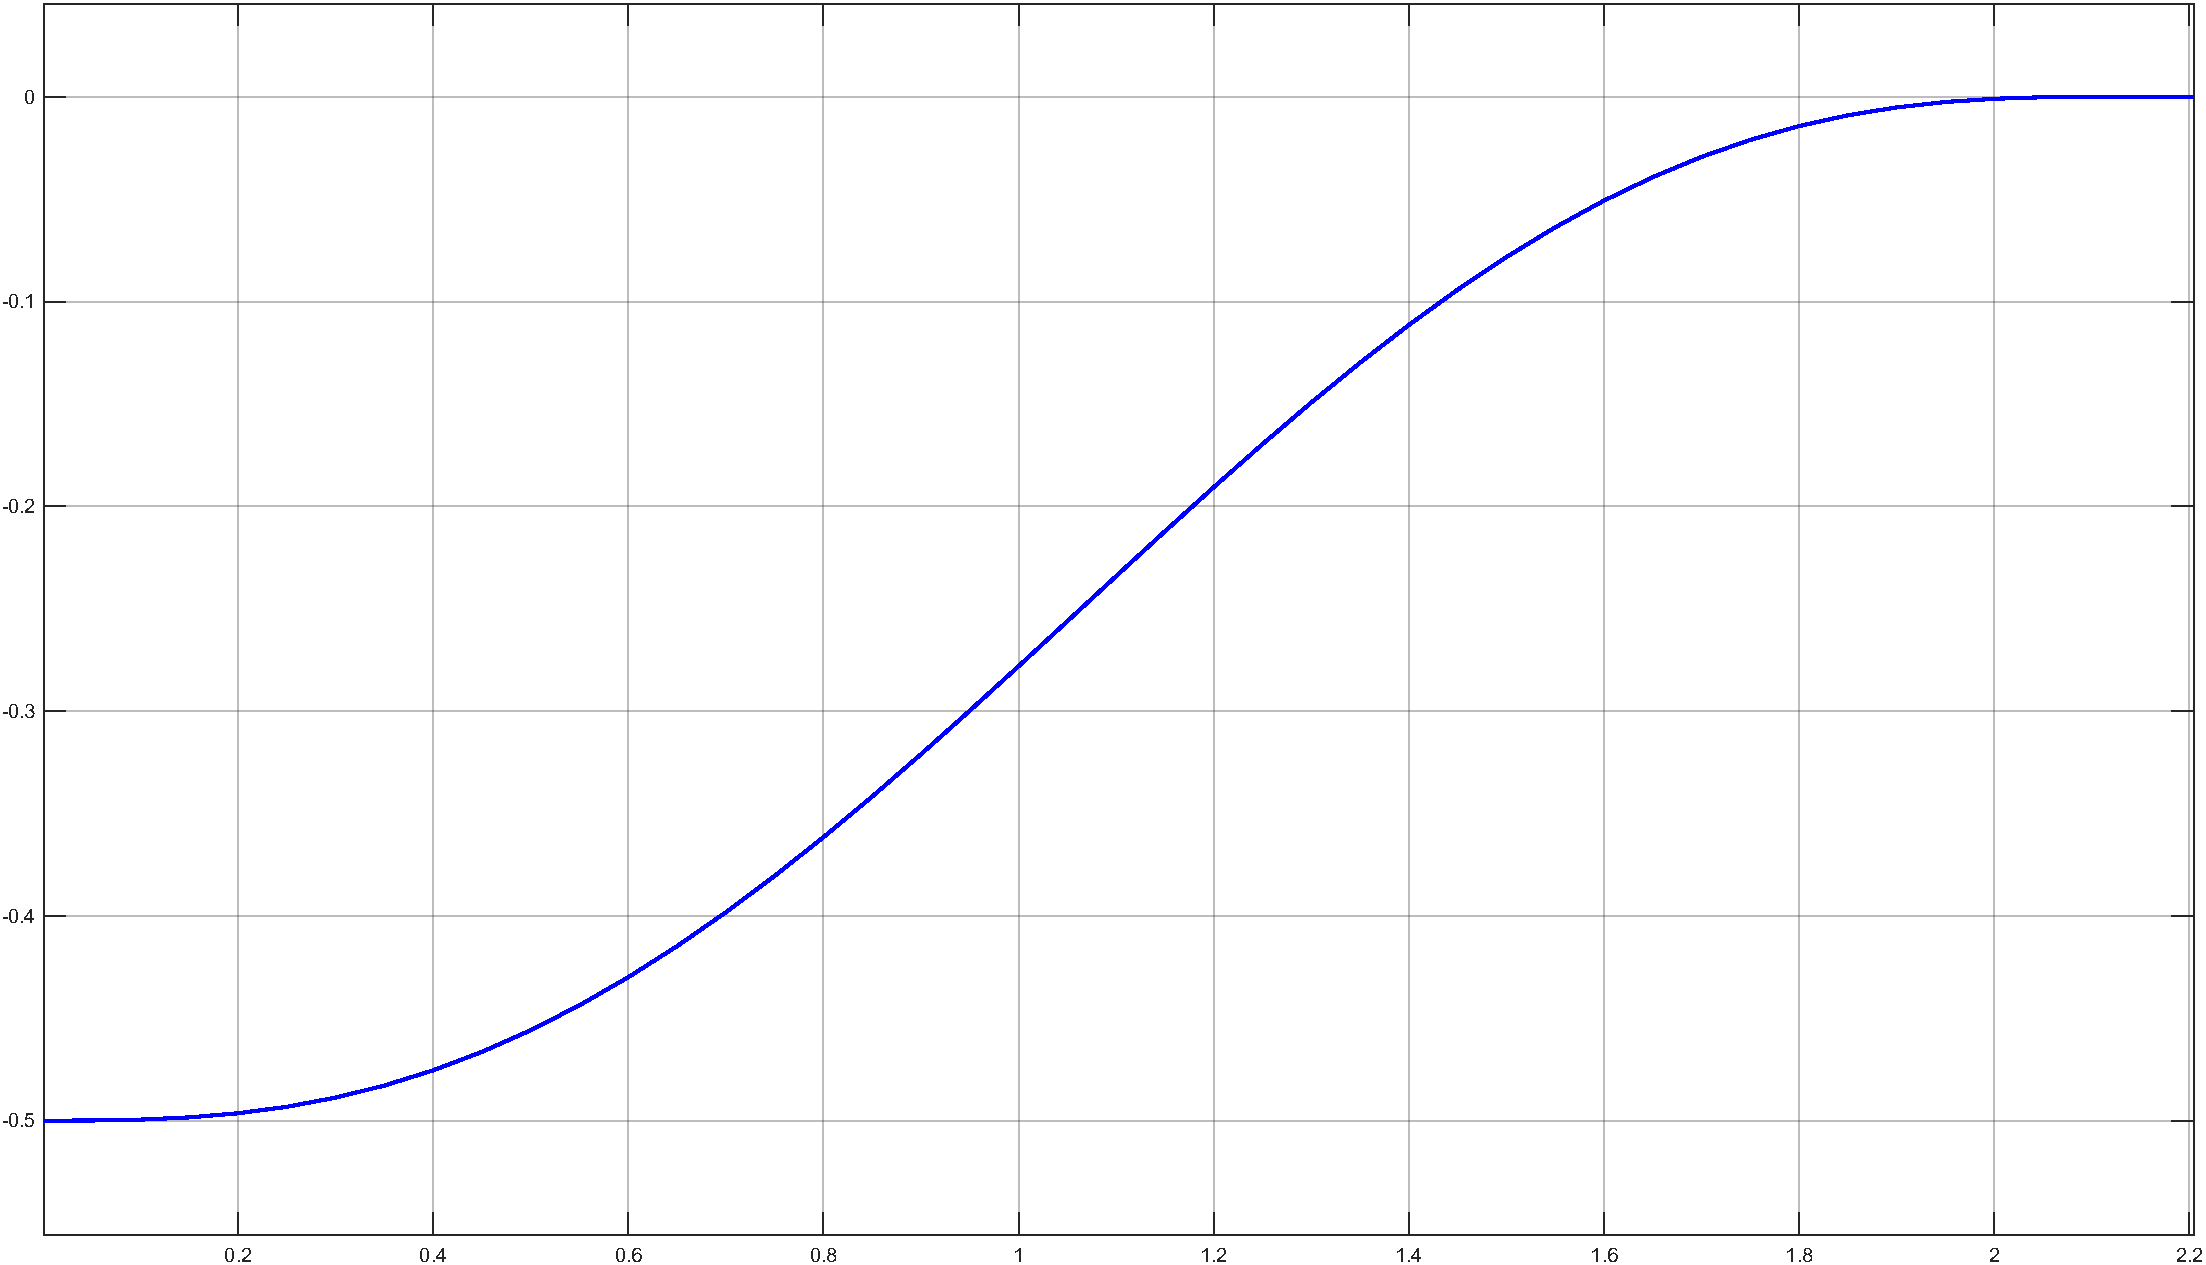
\includegraphics[width=0.8\textwidth]{images/4_NMPC_Trajectory/MPC_TRAJ_REF.pdf}
    \caption{\rl{نمونه‌ای از پروفایل مسیر مرجع نرم (\lr{S-Curve}) تولید شده توسط برنامه‌ریز سینماتیکی برای جابجایی $0.5$ متر.}}
    \label{fig:trajectory_ref}
\end{figure}

همان‌طور که در شکل \ref{fig:trajectory_ref} مشاهده می‌شود، با به‌کارگیری این برنامه‌ریز، خطای موقعیت در هر گام زمانی بسیار ناچیز و در محدوده خطی باقی می‌ماند. این پروفایل سینماتیکی به عنوان ورودی مرجع به سیستم کنترل تزریق می‌شود تا کالسکه با رعایت محدودیت‌های فیزیکی، به نرمی شتاب گرفته و در زمان مشخص به هدف برسد. در فصل‌های آتی، این مسیر مرجع به عنوان شالوده اصلی در طراحی کنترل‌کننده‌های ردیاب مورد استفاده قرار می‌گیرد.